% Options for packages loaded elsewhere
\PassOptionsToPackage{unicode}{hyperref}
\PassOptionsToPackage{hyphens}{url}
%
\documentclass[
]{article}
\usepackage{amsmath,amssymb}
\usepackage{lmodern}
\usepackage{iftex}
\ifPDFTeX
  \usepackage[T1]{fontenc}
  \usepackage[utf8]{inputenc}
  \usepackage{textcomp} % provide euro and other symbols
\else % if luatex or xetex
  \usepackage{unicode-math}
  \defaultfontfeatures{Scale=MatchLowercase}
  \defaultfontfeatures[\rmfamily]{Ligatures=TeX,Scale=1}
  \setmainfont[]{SourceSansPro}
\fi
% Use upquote if available, for straight quotes in verbatim environments
\IfFileExists{upquote.sty}{\usepackage{upquote}}{}
\IfFileExists{microtype.sty}{% use microtype if available
  \usepackage[]{microtype}
  \UseMicrotypeSet[protrusion]{basicmath} % disable protrusion for tt fonts
}{}
\makeatletter
\@ifundefined{KOMAClassName}{% if non-KOMA class
  \IfFileExists{parskip.sty}{%
    \usepackage{parskip}
  }{% else
    \setlength{\parindent}{0pt}
    \setlength{\parskip}{6pt plus 2pt minus 1pt}}
}{% if KOMA class
  \KOMAoptions{parskip=half}}
\makeatother
\usepackage{xcolor}
\usepackage[margin=1in]{geometry}
\usepackage{graphicx}
\makeatletter
\def\maxwidth{\ifdim\Gin@nat@width>\linewidth\linewidth\else\Gin@nat@width\fi}
\def\maxheight{\ifdim\Gin@nat@height>\textheight\textheight\else\Gin@nat@height\fi}
\makeatother
% Scale images if necessary, so that they will not overflow the page
% margins by default, and it is still possible to overwrite the defaults
% using explicit options in \includegraphics[width, height, ...]{}
\setkeys{Gin}{width=\maxwidth,height=\maxheight,keepaspectratio}
% Set default figure placement to htbp
\makeatletter
\def\fps@figure{htbp}
\makeatother
\setlength{\emergencystretch}{3em} % prevent overfull lines
\providecommand{\tightlist}{%
  \setlength{\itemsep}{0pt}\setlength{\parskip}{0pt}}
\setcounter{secnumdepth}{-\maxdimen} % remove section numbering
\ifLuaTeX
  \usepackage{selnolig}  % disable illegal ligatures
\fi
\IfFileExists{bookmark.sty}{\usepackage{bookmark}}{\usepackage{hyperref}}
\IfFileExists{xurl.sty}{\usepackage{xurl}}{} % add URL line breaks if available
\urlstyle{same} % disable monospaced font for URLs
\hypersetup{
  pdftitle={Практическая работа 4. Генерация распределений. Проверка определений известных распределений},
  pdfauthor={Юрченков Иван Александрович, ассистент кафедры ПМ},
  hidelinks,
  pdfcreator={LaTeX via pandoc}}

\title{Практическая работа 4. Генерация распределений. Проверка
определений известных распределений}
\author{Юрченков Иван Александрович, ассистент кафедры ПМ}
\date{2022-10-19}

\begin{document}
\maketitle

\hypertarget{ux43fux43eux441ux442ux430ux43dux43eux432ux43aux430-ux437ux430ux434ux430ux447ux438}{%
\section{\texorpdfstring{\textbf{Постановка
задачи}}{Постановка задачи}}\label{ux43fux43eux441ux442ux430ux43dux43eux432ux43aux430-ux437ux430ux434ux430ux447ux438}}

\begin{enumerate}
\def\labelenumi{\arabic{enumi}.}
\tightlist
\item
  \textbf{Сгенерировать выборку нормального распределения
  \(\ Y \sim N(\mu, \sigma^2)\ \) используя определение центральной
  предельной теоремы}.
\end{enumerate}

\begin{center}\rule{0.5\linewidth}{0.5pt}\end{center}

\textbf{Важно}. Здесь и далее во всех заданиях слова \emph{случайная
реализация случайной величины, распределенной по какому-либо
распределению} обозначают вектор с конечным числом значений,
сгенерированный из соотвествующего распределения. То есть, если например
\(\ Y \sim N(\mu, \sigma^)\ -\) случайная реализация нормально
распределенной величины с параметрами \(\ \Theta = (\mu,\ \sigma^2)\ \),
то \(\ Y\ -\) это вектор из \(\ K\ \) значений
\(\ Y = (y_1, y_2, \dots, y_K)\ \), сгенирированный из нормального
распределения c заданными конкретными значениями параметров.

\begin{center}\rule{0.5\linewidth}{0.5pt}\end{center}

\begin{itemize}
\tightlist
\item
  На основе \(\ n \approx 10\div 20\ \) равномерно распределенных
  случайных реализаций случайных величин образовать новую выборку по
  определению центральной предельной теоремы.
\end{itemize}

Если \(\ Y_{i} \sim U(a_i, b_i), \ i = 1, 2, \dots, n\ \), где
\(\ Y_{i}\ -\) случайная реализация равномерно распределенной случайной
величины с параметрами \(\ a_i \in \mathbb{R},\ b_i \in \mathbb{R}\ \),
то ожидаемая нормально распределенная величина \(\ Y\ \) будет найдена
как:

\[
Y = \sum_{i=1}^{n} Y_i, \ i=1,2,\dots, n
\]

\begin{itemize}
\item
  Для получившейся выборки построить гистограмму, визуализировать на
  гистограмме теоретическую плотность нормального распределения по
  несмещенным точечным оценкам \(\ \hat{\mu}, \hat{\sigma}\ \).
\item
  Провести тест на нормальное распределение с помощью критерия
  \(\ \chi^2\)-Пирсона. Степени свободы рассчитывать как \(\ k = n\ \).
\item
  Качественно определить влияние числа сгенерированных равномерно
  распределенных величин на итоговое качество генерации нормального
  распределения при помощи взятия 3 тестовых генераций при разных \(n\)
  и проведения теста на распределение.
\end{itemize}

Для генерации выборок рекомендуется пользоваться встроенными в
компьютерные статистические пакеты функциями генерации
\textbf{равномерно распределённых случайных величин}, которые задаются с
помощью параметров границ интервала генерации чисел \(a\) и \(b\).

\begin{enumerate}
\def\labelenumi{\arabic{enumi}.}
\setcounter{enumi}{1}
\tightlist
\item
  \textbf{Сгенерировать выборку \(\ \chi^2\)-распределения
  \(\ R \sim \chi_{k}^2\ \) используя определение распределения
  \(\ \chi^2\ \)}.
\end{enumerate}

\begin{itemize}
\tightlist
\item
  На основе \(\ Z\)-оценок случайных реализаций нормально распределенных
  случайных величин \(\ L_{i} \sim N(\mu_i, \sigma_i^2)\ \) образовать
  новую выборку по определению \(\ \chi^2\)-распределения:
\end{itemize}

\[
R = \sum_{i = 1}^{n} Z[L_i]^2,\ \ Z[L_i] = \frac{L - E[L]}{\sigma[L]}, \ L_i \sim N(\mu_i, \sigma_i^2),\ i = 1,2,\dots,n
\]

\begin{itemize}
\item
  Для получившейся выборки построить гистограмму, визуализировать на
  гистограмме теоретическую плотность \(\ \chi_k^2\ \) распределения c
  \(\ k = n\ \) степенями свободы.
\item
  Провести тест на \(\ \chi^2\ \) с помощью критерия
  \(\ \chi^2\)-Пирсона.
\end{itemize}

Для генерации \textbf{нормально распределенных реализаций} случайных
величин рекомендуется пользоваться встроенными в статистические пакеты
функциями для генерации значений выборки из нормального распределения,
которые задаются с помощью параметров математического ожидания \(\mu\) и
стандатрного отклонения \(\sigma^2\).

\begin{enumerate}
\def\labelenumi{\arabic{enumi}.}
\setcounter{enumi}{2}
\tightlist
\item
  \textbf{Сгенерировать выборку распределения Фишера на основе
  определения}.
\end{enumerate}

\begin{itemize}
\tightlist
\item
  На основе двух случайных реализаций \(\ Y_1, Y_2\ \) случайных
  величин, распределенных по \(\chi^2\)-распределению со степенями
  свободы \(\ d_1, d_2\ \) соответственно, сгенерировать выборку,
  распределенную по распределению Фишера \(\ S \sim F(d_1, d_2)\ \) в
  соответствии с определением:
\end{itemize}

\[
S = \frac{Y_1 / d_1}{Y_2 / d_2}, \ S\sim F(d_1, d_2).
\]

\begin{itemize}
\item
  Для получившейся выборки построить гистограмму, визуализировать на
  гистограмме теоретическую плотность \(\ F(d_1, d_2)\ \) распределения.
\item
  Провести тест на распределение Фишера с помощью критерия
  \(\ \chi^2\)-Пирсона.
\end{itemize}

Для генерации выборки фиксированного размера из распределения \(\chi^2\)
рекомендуется пользоваться встроенными в статистические пакеты функциями
для генерации случайных выборок из распределения \(\chi^2\) с \(df\)
степенями свободы.

\begin{enumerate}
\def\labelenumi{\arabic{enumi}.}
\setcounter{enumi}{3}
\tightlist
\item
  \textbf{Сгенерировать выборку t-распределения на основе определения}.
\end{enumerate}

\begin{itemize}
\tightlist
\item
  На основе \(\ n \approx 2\div 8\ \) случайных реализаций
  \(\ Y_1, Y_2, \dots, Y_n\ \) случайных величин, распределенных по
  стандартному нормальному распределению
  \(\ Y_i \sim N(0, 1), \ i = 1, 2, \dots, n\ \), сгенерировать выборку
  \(\ T \sim t(n)\ \), распределенную по \(t\)-распределению Стьюдента с
  \(\ df = n\ \) степенями свободы в соответствии с определением:
\end{itemize}

\[
T = \frac{Y_0}{\sqrt{\frac{1}{n} \sum_{i=1}^{n} Y_i^2}}, \quad Y_0 \sim N(0, 1).
\]

\begin{itemize}
\tightlist
\item
  Реализовать вычисление аналитической плотности \(t\)-распределения
  Стьюдента с использованием бета-функции:
\end{itemize}

\[
{\displaystyle p_{t}(x\ |\ n)={\frac {1}{{\sqrt {n}}\,\mathrm {B} ({\frac {1}{2}},{\frac {n}{2}})}}\left(1+{\frac {x^{2}}{n}}\right)^{\!-{\frac {n+1}{2}}}},
\] где

\[
{\displaystyle \mathrm {B} (x,y)=\int \limits _{0}^{1}t^{x-1}(1-t)^{y-1}\,dt,}
\]

определённая при \({\displaystyle \operatorname {Re} x>0}\),
\({\displaystyle \operatorname {Re} y>0}\).

\begin{itemize}
\item
  Для получившейся выборки построить гистограмму, визуализировать на
  гистограмме теоретическую плотность \(\ t(n)\ \).
\item
  Для получившейся выбрки провести тест на \(t\)-распределение Стьюдента
  с помощью критерия \(\ \chi^2\)-Пирсона, используя в качестве функции
  вероятности распределения \(\ P_t(x\ |\ n)\):
\end{itemize}

\[
P_t(x\ |\ n) = \int_{-\infty}^{x} p_t(z\ |\ n) dz.
\]

\begin{enumerate}
\def\labelenumi{\arabic{enumi}.}
\setcounter{enumi}{4}
\tightlist
\item
  Для всех заданий количество генерируемых значений выборки установить
  равным \(N \approx 100 \div 1000\). Уровень надежности для критерия
  \(\chi^2\)-Пирсона или метода анаморфоз \(\gamma = 0.95\).
\end{enumerate}

\hypertarget{ux43fux440ux438ux43cux435ux440-ux433ux435ux43dux435ux440ux430ux446ux438ux438-ux440ux430ux441ux43fux440ux435ux434ux435ux43bux435ux43dux438ux439}{%
\section{\texorpdfstring{\textbf{Пример генерации
распределений}}{Пример генерации распределений}}\label{ux43fux440ux438ux43cux435ux440-ux433ux435ux43dux435ux440ux430ux446ux438ux438-ux440ux430ux441ux43fux440ux435ux434ux435ux43bux435ux43dux438ux439}}

\hypertarget{ux433ux435ux43dux435ux440ux430ux446ux438ux44f-ux43dux43eux440ux43cux430ux43bux44cux43dux43eux433ux43e-ux440ux430ux441ux43fux440ux435ux434ux435ux43bux435ux43dux438ux44f-ux438ux437-ux441ux443ux43cux43cux44b-ux441ux43bux443ux447ux430ux439ux43dux44bux445-ux440ux435ux430ux43bux438ux437ux430ux446ux438ux439-ux440ux430ux432ux43dux43eux43cux435ux440ux43dux43e-ux440ux430ux441ux43fux440ux435ux434ux435ux43bux435ux43dux43dux43eux439-ux441ux43bux443ux447ux430ux439ux43dux43eux439-ux432ux435ux43bux438ux447ux438ux43dux44b}{%
\subsection{\texorpdfstring{\textbf{1. Генерация нормального
распределения из суммы случайных реализаций равномерно распределенной
случайной
величины}}{1. Генерация нормального распределения из суммы случайных реализаций равномерно распределенной случайной величины}}\label{ux433ux435ux43dux435ux440ux430ux446ux438ux44f-ux43dux43eux440ux43cux430ux43bux44cux43dux43eux433ux43e-ux440ux430ux441ux43fux440ux435ux434ux435ux43bux435ux43dux438ux44f-ux438ux437-ux441ux443ux43cux43cux44b-ux441ux43bux443ux447ux430ux439ux43dux44bux445-ux440ux435ux430ux43bux438ux437ux430ux446ux438ux439-ux440ux430ux432ux43dux43eux43cux435ux440ux43dux43e-ux440ux430ux441ux43fux440ux435ux434ux435ux43bux435ux43dux43dux43eux439-ux441ux43bux443ux447ux430ux439ux43dux43eux439-ux432ux435ux43bux438ux447ux438ux43dux44b}}

Центральная предельная теорема напрямую утверждает о том, что случайная
величина, составленная в виде суммы \(S = Y_1 + Y_2 + \dots Y_n\)
сулчайных величин \(Y_i\) с конечным математическим ожиданием \(\mu\) и
дисперсией \(\sigma^2\), обладает свойством:

\[
  \frac{S - n\cdot \mu}{\sqrt{n} \cdot \sigma} \to N(0, 1), \quad n\rightarrow +\infty,
\] где \(N(0, 1)\ -\) стандартное нормальное распределение.

В другой формулировке теоремы говорится о сумме величин с конечным
\textbf{неодинаковым} математическим ожиданием \(\mu_i\) и стандарным
отклонением \(\sigma_i\) для каждого члена суммы
\(S = \sum_{i=1}^nY_i, \ i=1,2,\dots, n\).

\textbf{ЦПТ Линдеберга}

Пусть независимые случайные величины \(Y_{1},\ldots ,Y_{n},\ldots\)
определены на одном и том же вероятностном пространстве и имеют конечные
математические ожидания и дисперсии:
\({\mathbb {E}}[X_{i}]=\mu _{i},\;{\mathrm {D}}[X_{i}]=\sigma _{i}^{2}\).

Пусть \(S_{n}=\sum \limits _{i=1}^{n}X_{i}\).

Тогда
\({\mathbb {E}}[S_{n}]=m_{n}=\sum \limits_{{i=1}}^{n}\mu_{i},\;{\mathrm {D}}[S_{n}]=s_{n}^{2}=\sum \limits_{{i=1}}^{n}\sigma _{i}^{2}\).

И пусть выполняется условие Линдеберга:

\[
\forall \varepsilon >0,\;\lim \limits _{{n\to \infty }}\sum \limits _{{i=1}}^{n}{\mathbb {E}}\left[{\frac {(Y_{i}-\mu _{i})^{2}}{s_{n}^{2}}}\,{\mathbf {1}}_{{\{|X_{i}-\mu _{i}|>\varepsilon s_{n}\}}}\right]=0,
\] где \({\mathbf {1}}_{{\{|X_{i}-\mu _{i}|>\varepsilon s_{n}\}}}\)
функция --- индикатор.

Тогда

\[
{\frac {S_{n}-m_{n}}{s_{n}}}\to N(0,1)
\]

по распределению при \(n\to \infty\).

В простыми словами, данная формулировка ЦПТ говорит о том, что если
сумма математических ожиданий квадратов \(z\)-оценок случайных величин
\(Y_i, \ i=1,2,\dots n\) в определенной окрестности в предеде
\(n \to +\infty\) стремится к нулю, то составленная случайная величина:

\[
S = \sum_{i=1}^{n} Y_i \sim N\left(\mu =\sum_{i=1}^n \mu_i, \sigma^2 = \sum_{i=1}^{n} \sigma_i^2\right),
\] будет распределена нормально с математическим ожиданием
\(\mu = \sum_{i=1}^n \mu_i\) и стандартным отклонением
\(\sigma^2 = \sum_{i=1}^{n} \sigma_i^2\).

Сгенерировав \(n\) равномерных распределений
\(Y_i \sim Uniform(a_i, b_i), \ (a_i, b_i) \ in \mathbb{R}\)
распределений, отобразим гистограмму полученной суммы их реализаций как
отдельной случайной величины. На итоговом графике также отобразим
\(\mu\) и \(\mu + (-3\sigma, -2\sigma, \dots, 3\sigma)\) значения,
полученные напрямую из определения выше, изобразив их штриховой линией.

\begin{center}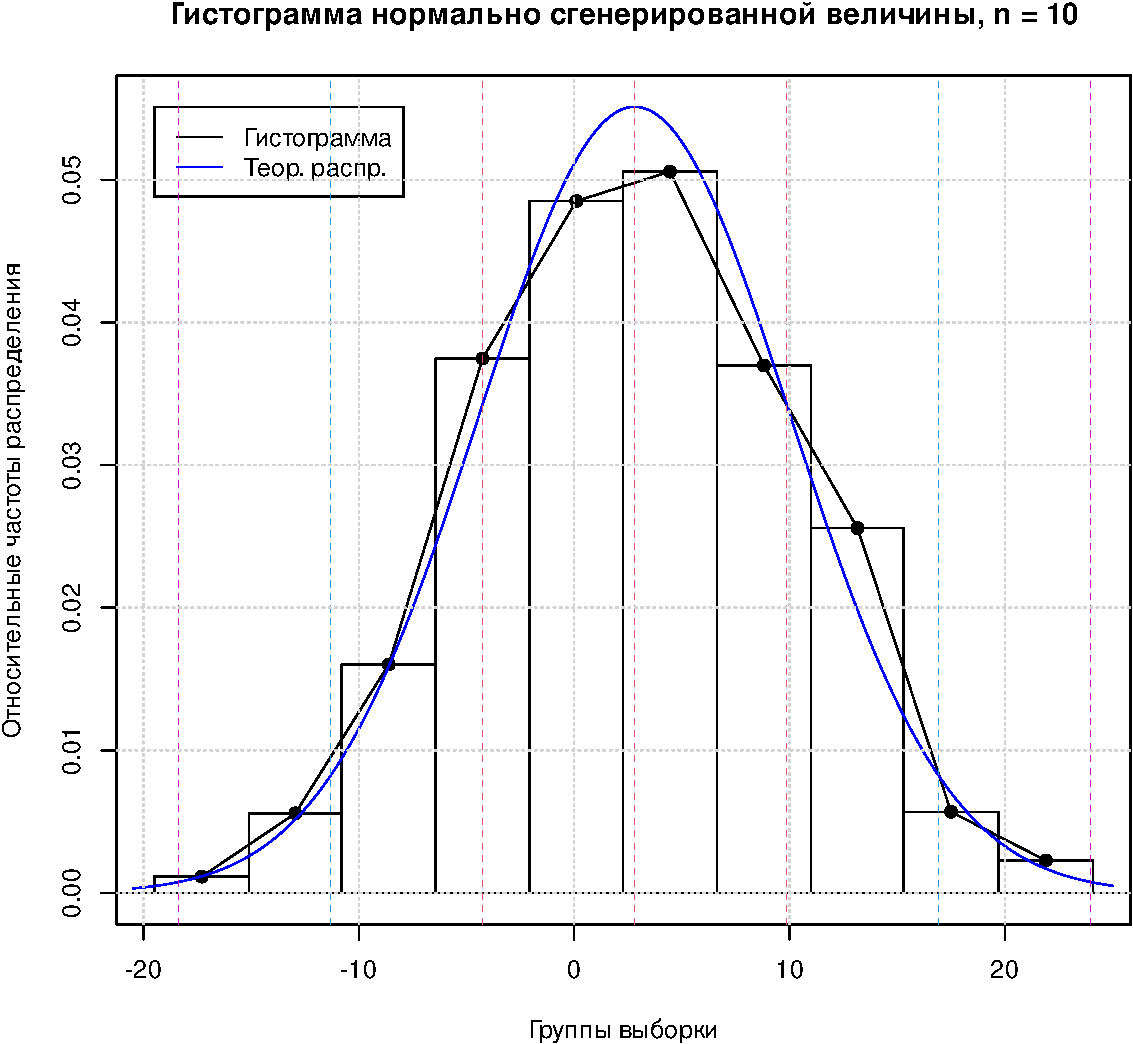
\includegraphics[width=0.6\linewidth]{Prac4_files/figure-latex/unnamed-chunk-3-1} \end{center}

Полученную гистограмму по её оцененным \(\mu\) и \(\sigma^2\) отобразим
в спрямляющих координатах нормального распределения, где по оси \(x\)
отложены теоретические значения вероятности получения тех же значений,
что и в исходной гистограмме, а по оси \(y\) отобразим сгенерированные
значения относительных частот при тех же значениях выборки и биссекрису.

\begin{center}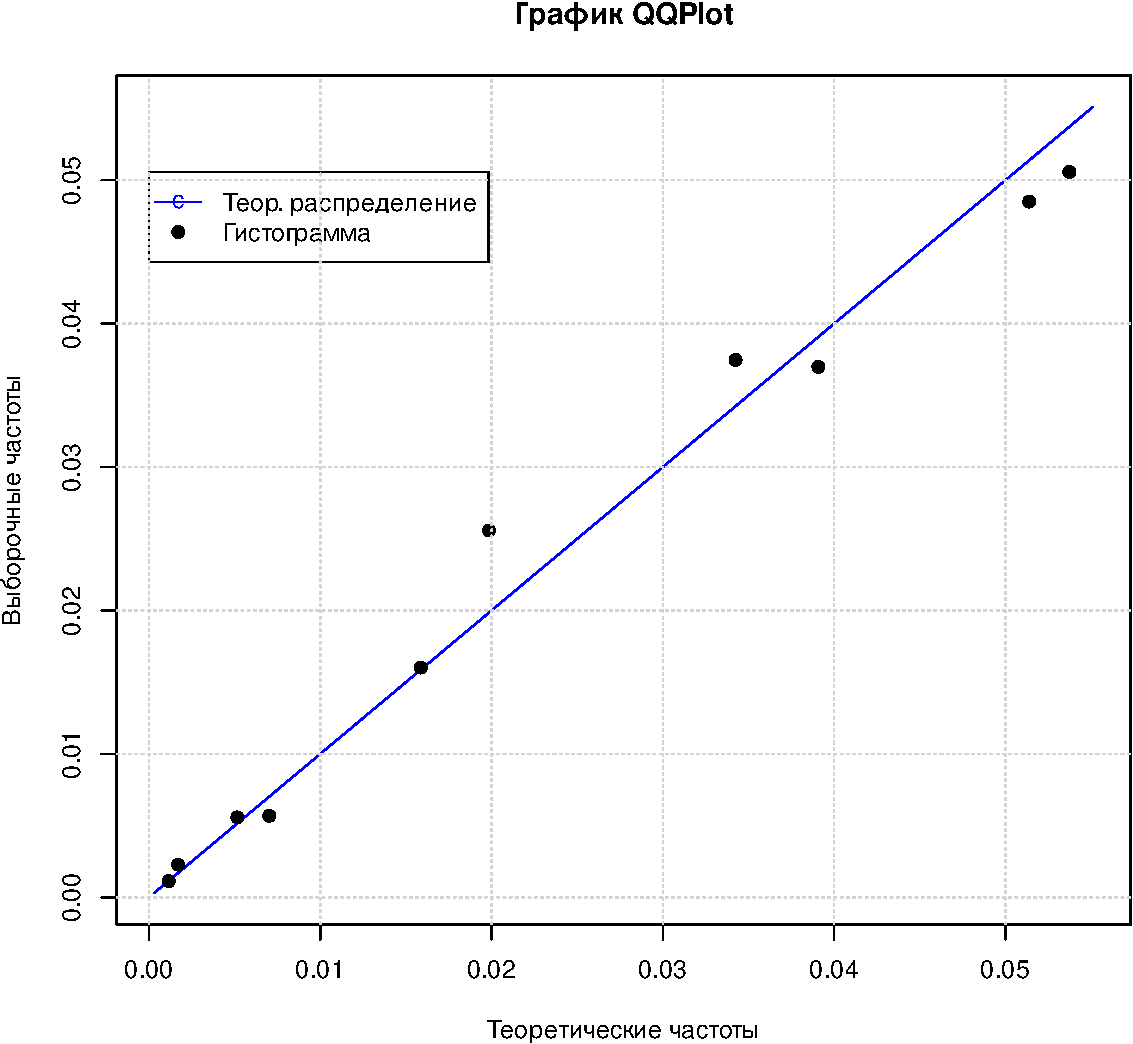
\includegraphics[width=0.6\linewidth]{Prac4_files/figure-latex/unnamed-chunk-4-1} \end{center}

По полученному спрямлению имеем возможность оценить близость полученных
зависимостей на основе коэффициента детерминации, посчитав его
относительно теоретической зависимости по оцененным параметрам
\(\hat{y} \sim N(\mu, \sigma^2)\) и практически полученных значений
относительных частот, деленных на ширину интервалов по гистограмме
\(y_i = p_i / h\):

\[
R^2(y, \hat{y}) = 1 - \frac{\sum \limits_{i=1}^{g} (\hat{y}_i - y_i)^2}{\sum \limits_{i=1}^{g} (\hat{y}_i - E[\hat{y}])^2}.
\]

Полученное значение коэффициента \(R^2(y, \hat{y})=\) 0.98, что можно
расценивать как положительный тест на нормальное распределение.

\hypertarget{ux433ux435ux43dux435ux440ux430ux446ux438ux44f-chi2-ux440ux430ux441ux43fux440ux435ux434ux435ux43bux435ux43dux438ux44f-ux43fux43e-ux43eux43fux440ux435ux434ux435ux43bux435ux43dux438ux44e}{%
\subsection{\texorpdfstring{\textbf{2. Генерация
\(\chi^2\)-Распределения по
определению}}{2. Генерация \textbackslash chi\^{}2-Распределения по определению}}\label{ux433ux435ux43dux435ux440ux430ux446ux438ux44f-chi2-ux440ux430ux441ux43fux440ux435ux434ux435ux43bux435ux43dux438ux44f-ux43fux43e-ux43eux43fux440ux435ux434ux435ux43bux435ux43dux438ux44e}}

Выборку реализации случайной величны распределенной по
\(\chi^2\)-распределению можно получить из его определения:

\[
S = \sum_{i=1}^{n} Z[Y_i]^2,\quad  Y_i \sim N(\mu_i, \sigma_i^2), \quad i=1,2,\dots,n,
\] где \(Z[Y_i]\ -\) это \(Z\)-оценки соответсвующей реализации
нормально распределенной случайной величины
\(Y_i \sim N(\mu_i, \sigma_i^2)\).

Таким образом выборку \(S\) мы можем получить сгенерировав \(n\) выборок
из нормального распределения \(N(\mu_i, \sigma_i^2)\) со случайными
параметрами \(\Theta = (\mu_i, \sigma_i^2)\), получив из \(Z\)-оценки и
сложив квадраты полученных значений выборок между собой соответственно.

Проделав такую процедуру получим гистограмму сгенерированной выборки, на
которую наложим визуализацию теоретических значений распределения
\(\chi^2\) со степенями свободы \(df = n\).

\begin{center}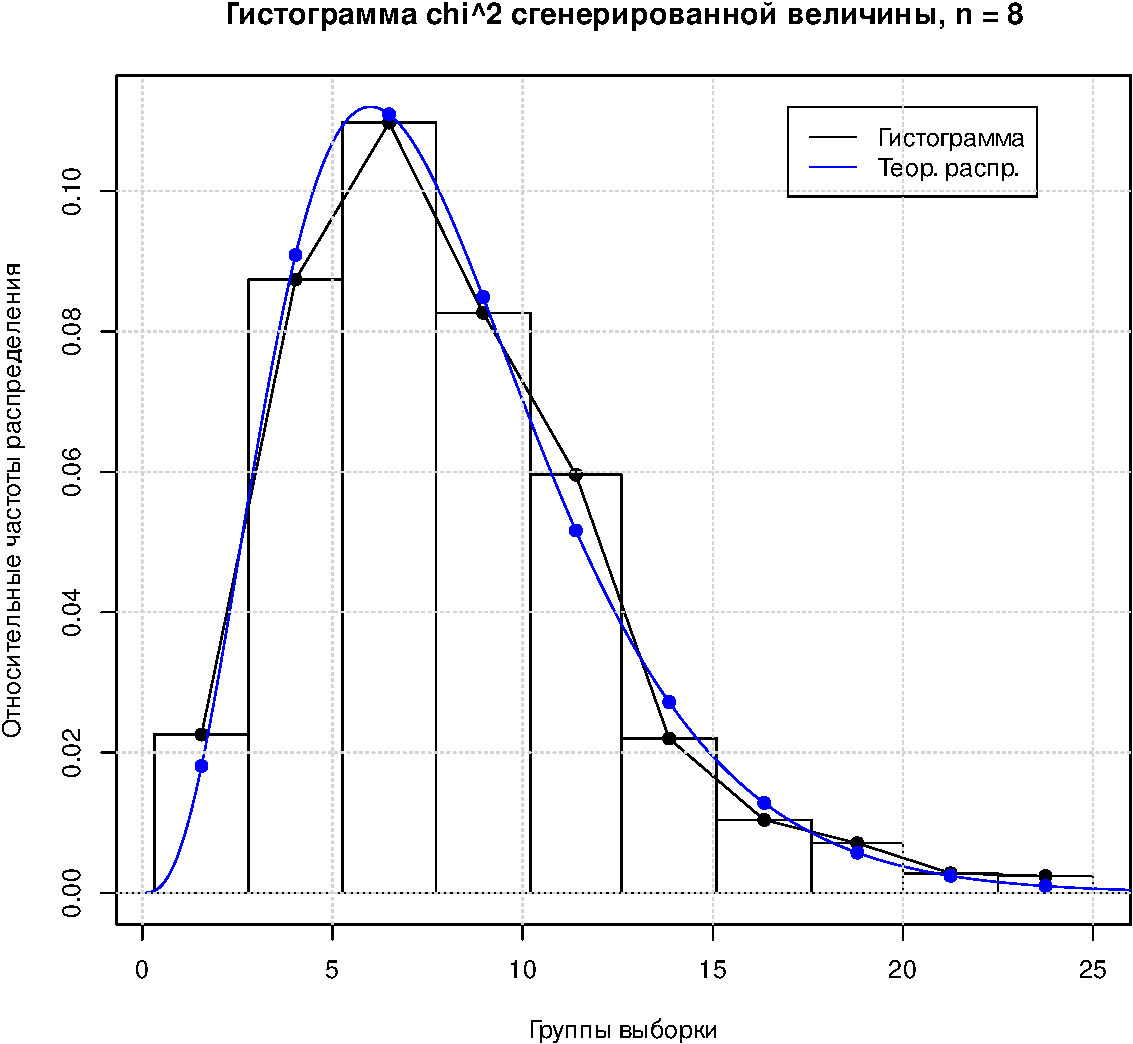
\includegraphics[width=0.6\linewidth]{Prac4_files/figure-latex/unnamed-chunk-5-1} \end{center}

Изобразим также этот график в новых координатах. Отложим по оси \(x\)
значения теоретической вероятности из функции плотности
\(\chi^2\)-распределения. По оси \(y\) отложим значения полученных
относительных частот сгенерированной выборки. Получим спрямление,
относительно линейности точек гистограммы которого можно судить о
принадлежности выборки распределению.

\begin{center}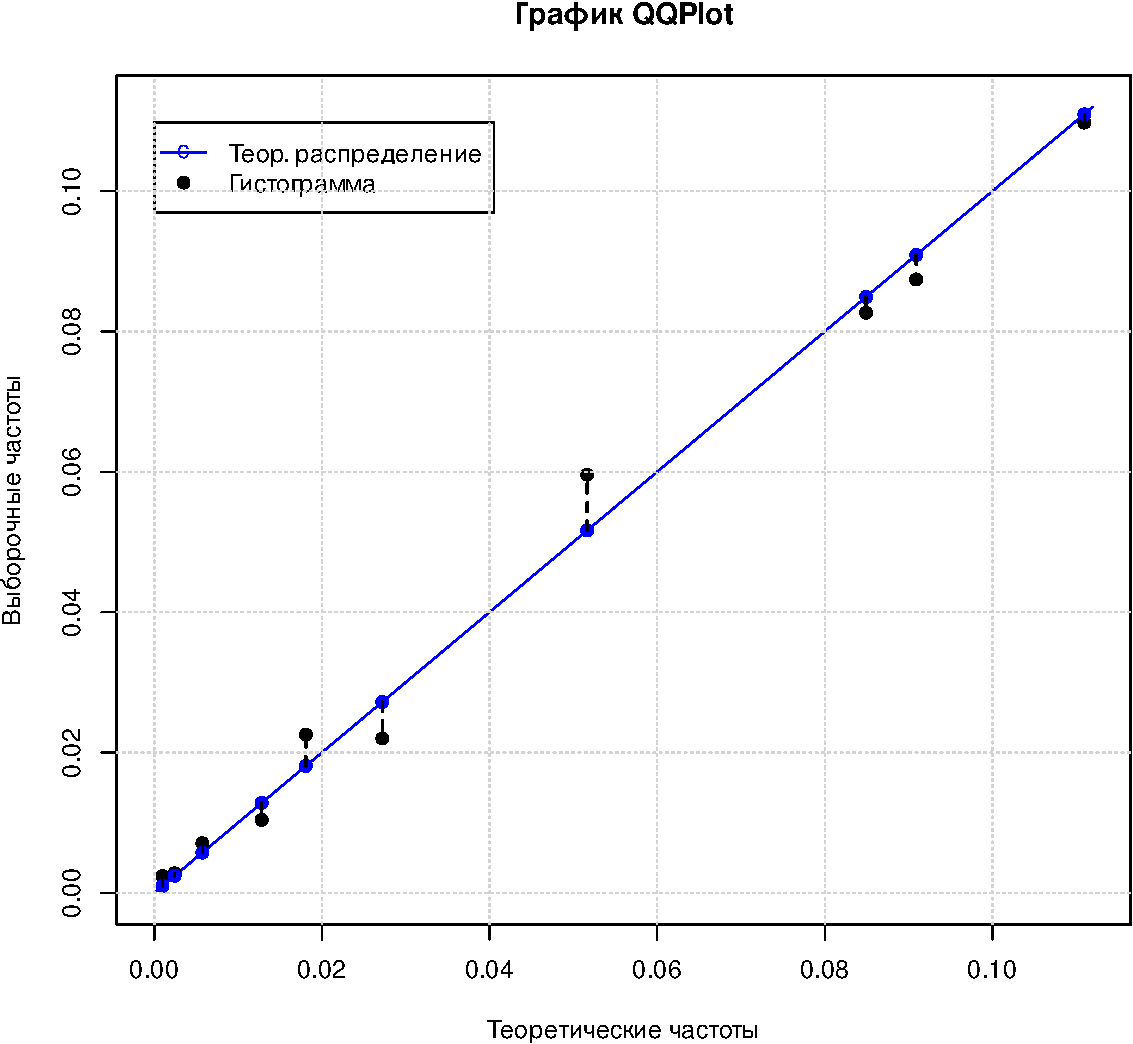
\includegraphics[width=0.6\linewidth]{Prac4_files/figure-latex/unnamed-chunk-6-1} \end{center}

Коэффициент детерминации между значениями теоретического распределения и
значениями частот гистограммы: \(R^2(y, \hat{y}) =\) 0.91. Значение
является довольно высоким, что можно расценивать как положительный тест.

\hypertarget{ux440ux435ux430ux43bux438ux437ux430ux446ux438ux44f-ux440ux430ux441ux43fux440ux435ux434ux435ux43bux435ux43dux438ux44f-ux444ux438ux448ux435ux440ux430-ux43fux43e-ux43eux43fux440ux435ux434ux435ux43bux435ux43dux438ux44e}{%
\subsection{\texorpdfstring{\textbf{3. Реализация распределения Фишера
по
определению}}{3. Реализация распределения Фишера по определению}}\label{ux440ux435ux430ux43bux438ux437ux430ux446ux438ux44f-ux440ux430ux441ux43fux440ux435ux434ux435ux43bux435ux43dux438ux44f-ux444ux438ux448ux435ux440ux430-ux43fux43e-ux43eux43fux440ux435ux434ux435ux43bux435ux43dux438ux44e}}

Распределение Фишера по определению является отношением реализаций двух
случаных величин из \(\chi^2\)-распределения:

\[
S = \frac{Y_1/d_1}{Y_2/d_2} \sim F(d_1, d_2),\ \ Y_1 \sim \chi_{d_1}^2, \ Y_2 \sim \chi_{d_2}^2.
\]

Таким образом, можно получить выборку, распределенную по распределению
Фишера \(S \sim F(d_1, d_2)\) c \(d_1\) и \(d_2\) степенями свободы
распределений выборок \(Y_1\) и \(Y_2\) соответственно.

Сгенерируем выборку на основе определения распределения Фишера при
попощи сгенерированных выборок из распределения \(\chi^2\) по \(N\)
значений с разными степенями свободы \(d_1 = 20\), \(d_2 = 9\):

\begin{center}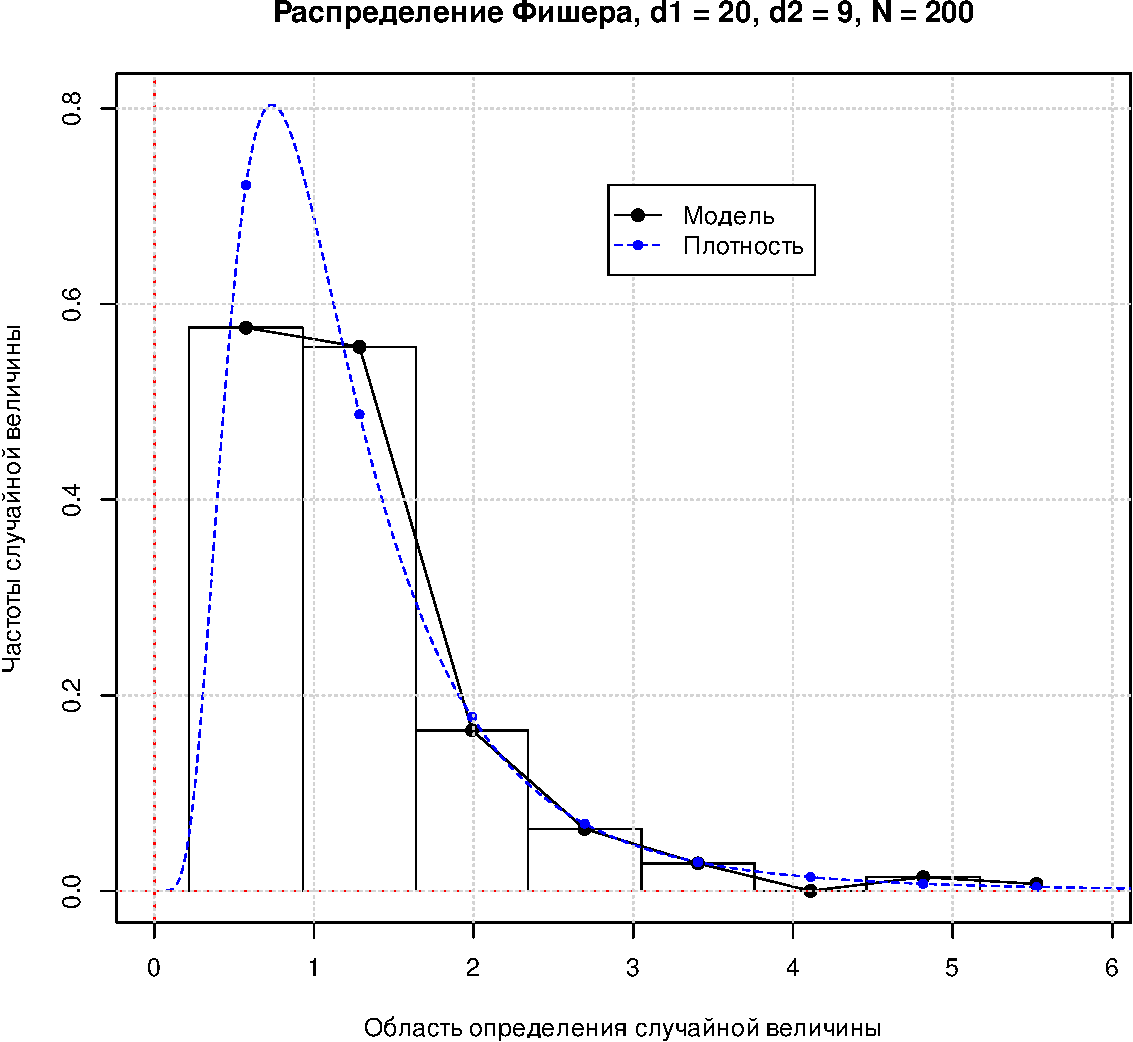
\includegraphics[width=0.6\linewidth]{Prac4_files/figure-latex/unnamed-chunk-7-1} \end{center}

Построим график в спрямляющих координатах по тому же принципу, что и
раньше, по оси абсцисс откладываем значения теоретической плотности
распределения Фишера, полученной при помощи встроенной в статистический
пакет функции, а по оси ординат откладываем сгенерированную выборку
распределения Фишера с \(d_1\) и \(d_2\) степенями свободы.

\begin{center}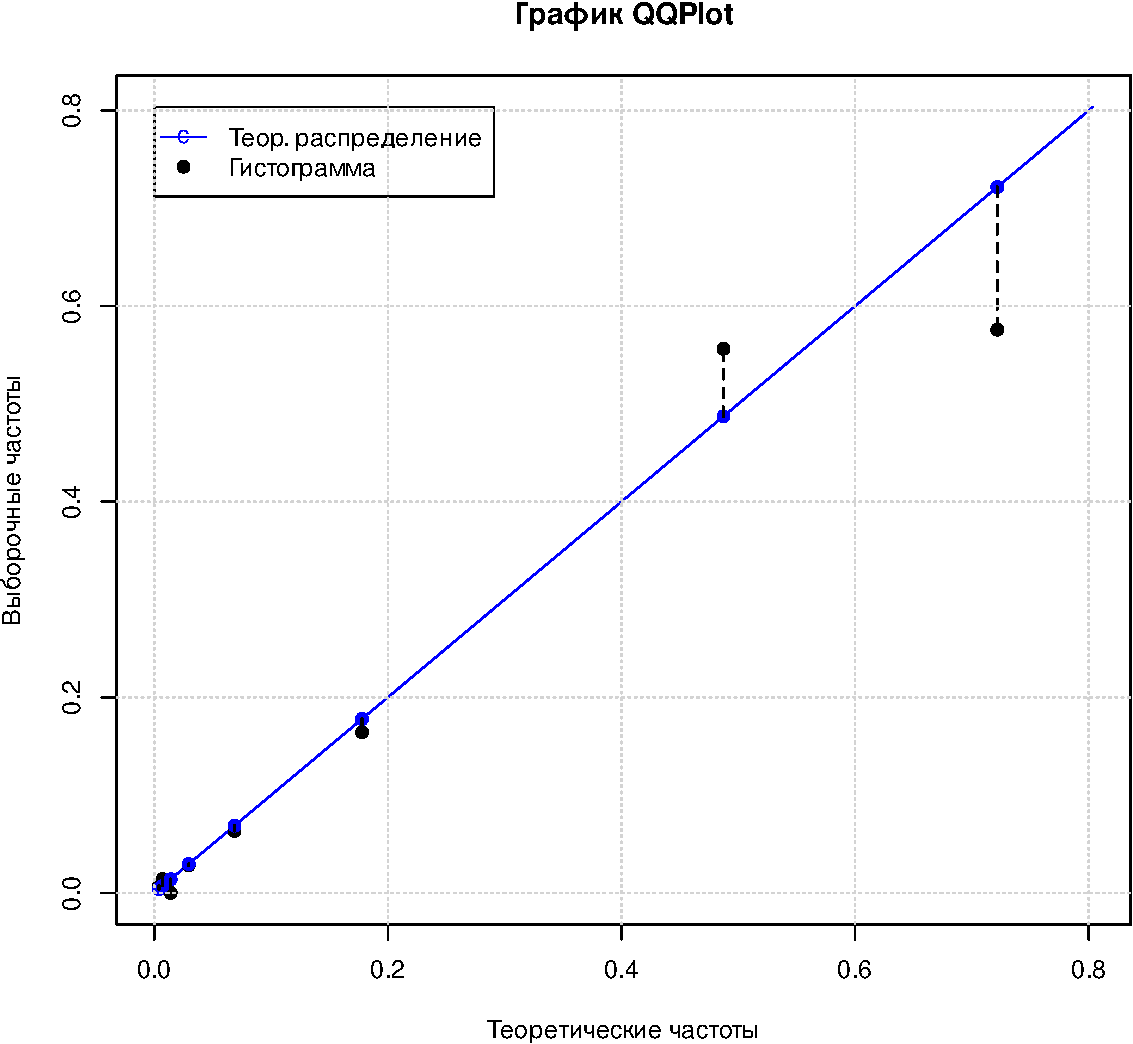
\includegraphics[width=0.6\linewidth]{Prac4_files/figure-latex/unnamed-chunk-8-1} \end{center}

По спрямлению можно оценить коэффициент детерминации между прямой и
данными и понять насколько зависимость близка к линейной, что будет
говорить о принадлежности выборки к полученному распределению:
\(R^2(y, \hat{y}) =\) 0.95. Значение является довольно высоким, что
можно расценивать как положительный тест.

\hypertarget{ux440ux435ux430ux43bux438ux437ux430ux446ux438ux44f-ux440ux430ux441ux43fux440ux435ux434ux435ux43bux435ux43dux438ux44f-ux441ux442ux44cux44eux434ux435ux43dux442ux430-ux43fux43e-ux43eux43fux440ux435ux434ux435ux43bux435ux43dux438ux44e}{%
\subsection{4. Реализация распределения Стьюдента по
определению}\label{ux440ux435ux430ux43bux438ux437ux430ux446ux438ux44f-ux440ux430ux441ux43fux440ux435ux434ux435ux43bux435ux43dux438ux44f-ux441ux442ux44cux44eux434ux435ux43dux442ux430-ux43fux43e-ux43eux43fux440ux435ux434ux435ux43bux435ux43dux438ux44e}}

Реализовав вычисление функции плотности для \(t\)-распределения
Стьюдента по формулам, мы имеем возможность отобразить на графике
полученные нами теоретические плотности распределения при разных
степенях свободы.

\begin{center}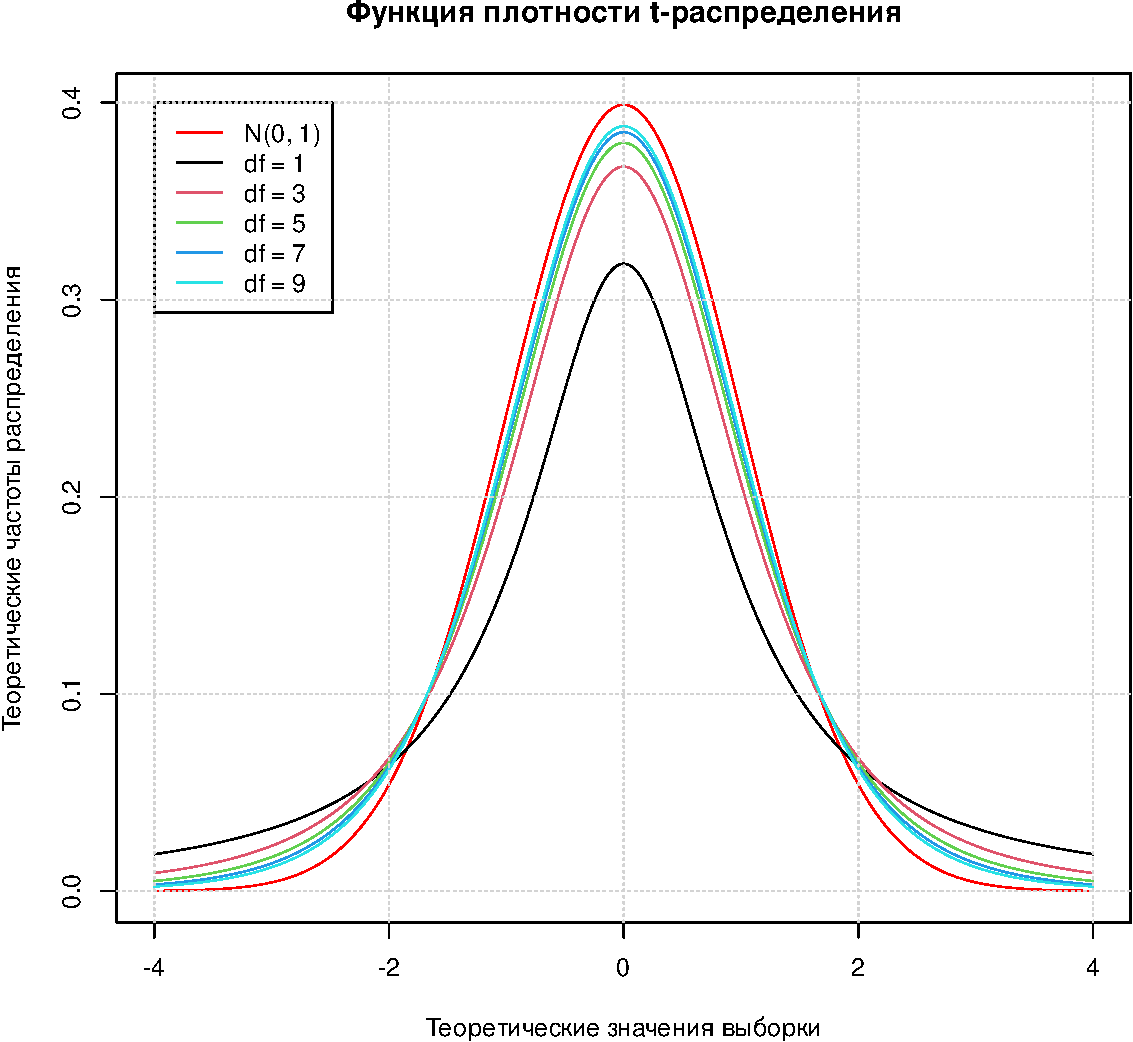
\includegraphics[width=0.6\linewidth]{Prac4_files/figure-latex/unnamed-chunk-9-1} \end{center}

На графике выше мы можем наблюдать сходимость графика плотности
\(t\)-распределения к стандартному нормальному распределению при
увеличении числа степеней свободы. Отсюда можно качественно делать вывод
о правдоподности аналитического определения плотности
\(t\)-распределения по формулам.

Попробуем сгенерировать выборку, удовлетворяющую \(t\)-распределению
Стьюдента с \(n\) степенями свободы. Для этого произведем генерацию
нормальных случайных величин в количестве равном \(n\) с выборками
количеством равным \(N\). Далее для еще одной сгенерированной
стандартной нормальной случайной величины произведем вычисления согласно
формулам и получим выборку, распределенную по \(t\)-распределению с
\(n\) степенями свободы:

\begin{center}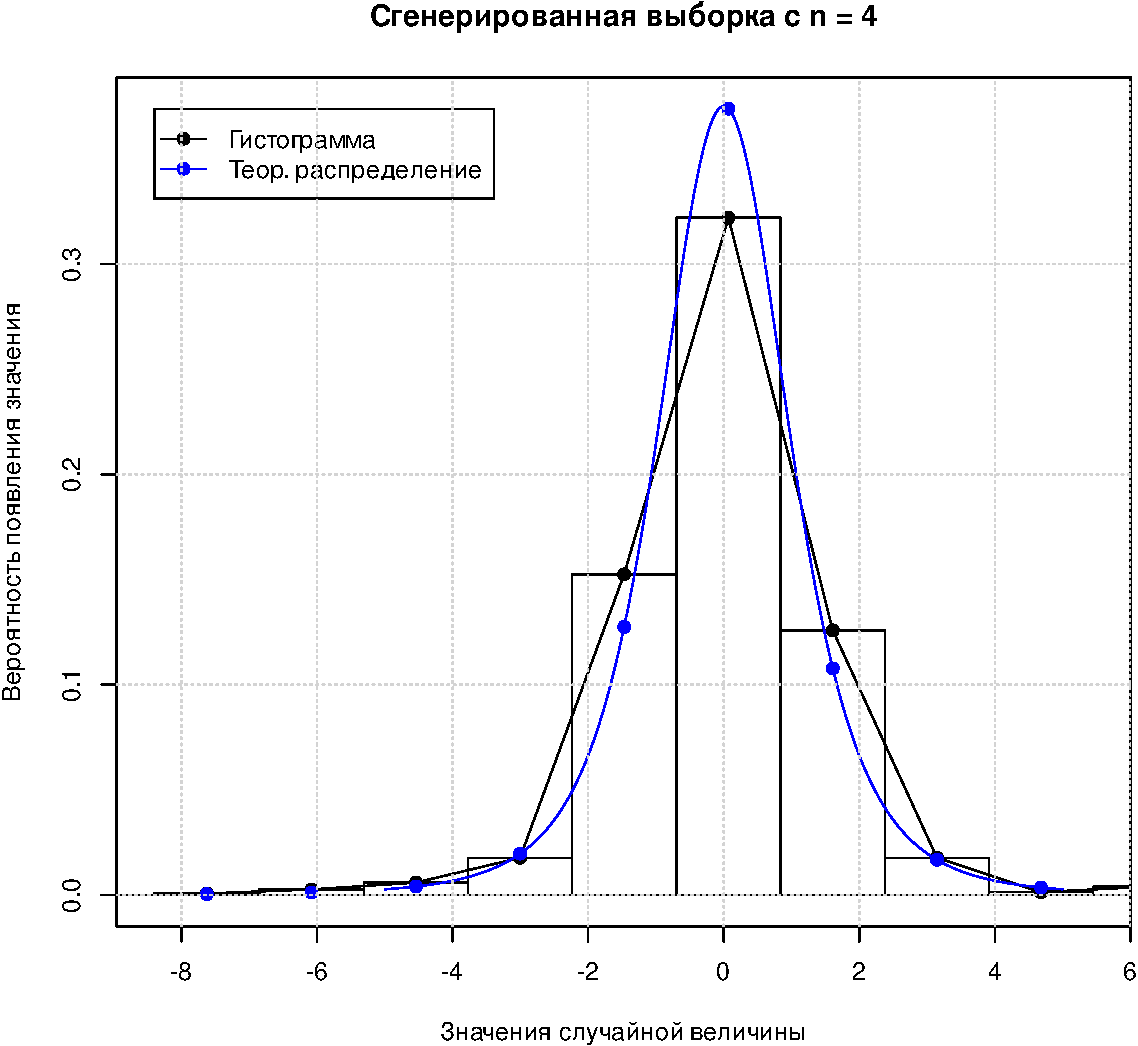
\includegraphics[width=0.6\linewidth]{Prac4_files/figure-latex/unnamed-chunk-10-1} \end{center}

Для полученных теоретических частот и гистограммы для сгенерированной
выборки построим график в координатах друг друга \(p_i \sim t(n)\) для
простой проверки на распределение. Спрямление получим:

\begin{center}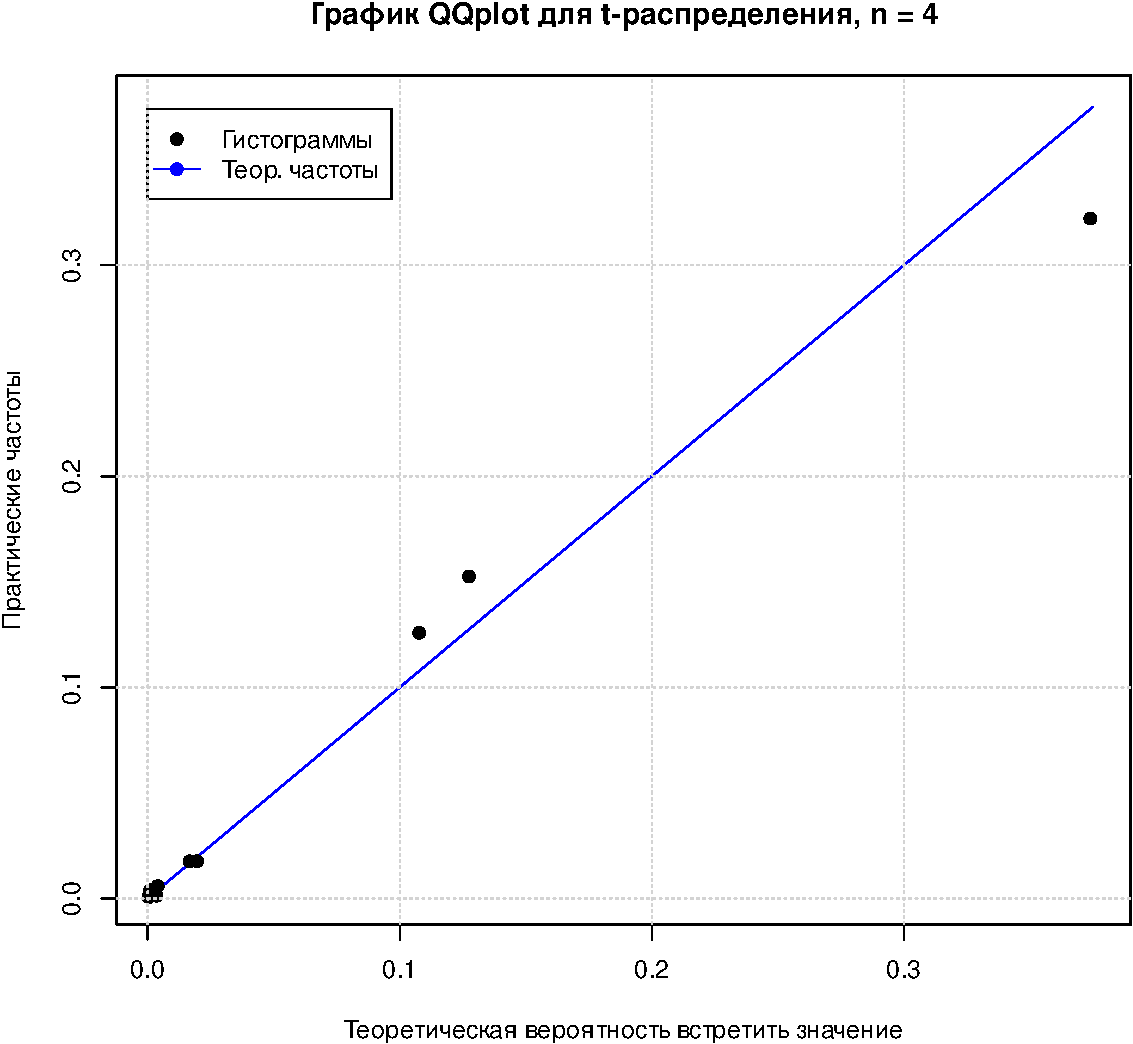
\includegraphics[width=0.6\linewidth]{Prac4_files/figure-latex/unnamed-chunk-11-1} \end{center}

И значение коэффициента детерминации: \(R^2(y, \hat{y}) =\) 0.979.
Значение \(R^2\) является довольно высоким, что можно расценивать как
положительный тест на распределение Стьюдента.

\hypertarget{ux432ux43eux43fux440ux43eux441ux44b-ux43dux430-ux437ux430ux449ux438ux442ux443-ux43fux440ux430ux43aux442ux438ux447ux435ux441ux43aux43eux439-ux440ux430ux431ux43eux442ux44b}{%
\section{\texorpdfstring{\textbf{Вопросы на защиту практической
работы}}{Вопросы на защиту практической работы}}\label{ux432ux43eux43fux440ux43eux441ux44b-ux43dux430-ux437ux430ux449ux438ux442ux443-ux43fux440ux430ux43aux442ux438ux447ux435ux441ux43aux43eux439-ux440ux430ux431ux43eux442ux44b}}

\begin{enumerate}
\def\labelenumi{\arabic{enumi}.}
\item
  Центральная предельная теорема. Реализации случайно распределенных
  величин. Независимые величины. Степени свободы суммы независимо
  распределенных величин.
\item
  Определение нормального распределения. Спрямление для координат
  нормального распределения. Определение параметров нормального
  распределения через точечные оценки. Определение параметров
  нормального распределения, образованного суммой независимых величин,
  через ЦПТ.
\item
  Определение распределения Фишера. Аналитические формулы
  математического ожидания и дисперсии расределения Фишера.
\item
  t-распределение Стьюдента. Аппроксимации и определение функции
  плотности. Смесь нормально расределенных величин. Определение
  \(Z\)-оценок.
\end{enumerate}

\end{document}
